\documentclass[conference]{IEEEtran}
\IEEEoverridecommandlockouts
% The preceding line is only needed to identify funding in the first footnote. If that is unneeded, please comment it out.
\usepackage{cite}
\usepackage{amsmath,amssymb,amsfonts}
\usepackage{algorithmic}
\usepackage{graphicx}
\usepackage[utf8x]{inputenc} 
\usepackage[OT1]{fontenc} 
\usepackage{textcomp}
\usepackage{xcolor}
\usepackage{mathtools}
\usepackage{subfig}

\def\BibTeX{{\rm B\kern-.05em{\sc i\kern-.025em b}\kern-.08em
    T\kern-.1667em\lower.7ex\hbox{E}\kern-.125emX}}
\begin{document}

\title{Understanding Image Advertisements and Predicting Sentiment\\}

\author{\IEEEauthorblockN{1\textsuperscript{st} Rohan Chopra}
\IEEEauthorblockA{\textit{40233019} \\
\textit{Concordia University}\\
Montreal, Canada \\
rohanchopra09@gmail.com}
\and
\IEEEauthorblockN{2\textsuperscript{nd} Harman Singh Jolly}
\IEEEauthorblockA{\textit{40204947} \\
\textit{Concordia University}\\
Montreal, Canada \\
jollyharmansingh@gmail.com}
}

\maketitle

\begin{abstract}
Promotion of products is now a common practice and is heavily controlled by broadcasting of advertisements. It is painstakingly difficult to personalize the content search by understanding the sentiments behind these image advertisements. It is proven that an image can be perceived in different manners and hence different emotions can be conveyed via them. This study tries to compare three backbone deep learning architectures on an advertisements dataset to potentioally classify the underlying sentiments interleaved in the images. 

Talk about F1 score, which model performed best amongst the tree, how grad-cam was applied in last layer to show the model reasoning.
\end{abstract}

\begin{IEEEkeywords}
component, formatting, style, styling, insert
\end{IEEEkeywords}

\section{Introduction}
In this fast paced world, companies now trade with the ever changing data we generate. With data, comes along user profiling or a set of topics that a user can be defined into. Perhaps, the  expansion of online visual content and social media has led to a surge of interest in the investigation of large-scale social multimedia analysis. In recent years, image advertisements have become increasingly prevalent in our daily lives. From billboards to social media ads, companies are constantly vying for our attention through visually appealing images. However, with the rise of sentiment analysis, it is now possible to predict the emotions that these images evoke in viewers. So, pondering over the platitude, `A picture says a thousand words' becomes necessary.

Tech giants like Facebook and Google have produced enormous wealth by advertisements only where 97.5\% of the \$116.6 billion generated by Facebook\cite{b1} and 70.9\% of Googles revenue\cite{b2} came in from broadcasting advertisements. Attracting customers to a product is a vital aspect of using  advertisements on both television and social media. Selection of ads by hand is a physically tedious and onerous job where provision of image based advertisements or videos becomes highly difficult via handpicking. So, automatic advertising techniques are developed, such as the contextual advertising method which aims to find the most relevant ad to a provided content without annoying customers.

The components that contribute to the effectiveness of these advertisements are intricate and are being analyzed in marketing science and consumer psychology. A particular focus of this research has been on comprehending the emotions and sentiments conveyed by visual media content, which has become increasingly popular for both academic and practical purposes. Sentiment analysis is a process of identifying and extracting opinions, emotions, and attitudes expressed in text. However, with the increasing use of visual media in advertising, there has been a need for sentiment analysis in images. Sentiment labels are used to annotate images with positive, negative or neutral sentiments. These annotations are used to train machine learning models to predict the emotions that an image is likely to evoke in viewers.
Powerful emotions conveyed by images and videos can amplify the message conveyed in the content, making it more impactful and capable of influencing the audience more effectively. But sometimes, advertisements aren’t able to hold viewers interest as the product shown doesn’t necessarily incline to the viewers choices or viewers actually skip watching advertisements that aren’t able to garner their attention, which is where a positive or a negative connotation comes into picture pertaining to sentiment of an advertisement.

Our report focuses on.


\section{Related Works}

In order to create an effective advertisement, researchers focus on tons of ideas to reach a balance of emotion and the type of message conveyed. The visual understanding or common sense that the “red color” symbolizes “stop” when used in traffic related series and symbolizes “blood” when used in medical related series is extremely potent in humans but negligible in computers. The recognition of non-photorealistic objects and symbolism are possible illustrations depicting the visual-rhetoric methods for conveying a message through ads. To fathom these rhetorics which not only requires the discernment of objects but also requires the decoding of this rhetoric \cite{b4}~\cite{b5}. Perhaps, a summarization about the image where it talks about \cite{b6}~\cite{b7} which objects are portrayed, how they are portrayed and answering the primal questions as to why they are portrayed. For instance, if an advertisement is meant to target a young audience, it can be designed with bright colors and positive sentiments to appeal to that demographic. On the other hand, an ad meant for an older audience may be designed with muted colors and neutral sentiments. By predicting the sentiments that an advertisement is likely to evoke, companies can tailor their ads to specific audiences, increasing their chances of success.

Exploring objects or generic nouns such as “cat” or “trees” have been a marvel of machine vision but the association of sentiments correlating to the visuals remains a challenging and seemingly insurmountable task. The difficulty of this endeavor stems from the significant emotional distance between the low visual characteristics and the high-level sentiment that adjectives convey. To fill this gap between visual characteristics and sentiments, Borth, Damian et al.\cite{b8} proposed an alternative method that represents sentiment-related visual concepts for an intermediary  representation. They have coined the term Adjective Noun Pairs (ANP) like “sprawling trees” or “sleepy cat” which are used to corroborate the adjective of nouns, further used to identify nouns. ANPs, despite not conveying emotions or sentiments explicitly, can still be effective indicators for identifying emotions portrayed in images, as they were identified based on a high correlation with emotion tags present in web photos. In their study Borth, Damian et al.\cite{b8} trained binary SVM classifiers on ANPs for whole images. To further enhance the classifiers, the authors Chen, Felix et al.\cite{b9} ncluded the localization of object-based concepts and the semantic similarity between these concepts in their work.

DeepSentiBank\cite{b10} hows significant efforts to interpret emotion from images using a model trained on web images that are tagged with multiple sentiments. Hussain, Zhang et al.\cite{b11} went further to apply DeepSentiBank and reached a conclusion to observe a detector for natural images (DeepSentiBank) couldn’t be applicable for advertisement images. Besides DeepsentiBank, Vedula \& Sun et al.\cite{b12} developed an advertisement recommendation system using sentiments in multimedia content. Using deep learning techniques, image and video analysis combined have garnered a great amount of headway for data analysis at Youtube and for contextual understanding in video advertising\cite{b13}. But, compared to other forms of media such as publishing or billboards, which are less personalized, a great deal of lacuna lies in interpreting advertisements media due to their extensive use of visual rhetoric as coined in Hussain, Zhang et al.\cite{b11}. 

An advertisement demands much in depth analysis due to the fact that they intend to persuade people for their motion by lobbying their product as best to make people aware of any social cause. Give an example of ad images here, some advertisement that represents a hidden social cause. The motive to persuade people is deeply imbibed inside an advertisement, where sometimes it is portrayed via simple tone or sometimes via sarcasm. In order to understand this underlying sentiment, only appearance isn’t enough. Therefore, to personalize the experience with ads, it is imperative to  not only understand its topic, but also the emotion it conveys. Zhang, Luo et al.\cite{b14} introduced a framework that amalgamates multiple modalities together for envisioning topic and sentiment related predictions to further conceptualize advertisements.

\section{Dataset} \label{sec:dataset}

We have used a publicly available dataset developed by the combined efforts by Hussain et al at the University of Pittsburgh with over 64,000 images including all sorts of ads. Amazon Mechanical Turk workers were asked to tag each advertisement to its respective topic (eg.\ any product targets which audience for broadcasting their product) and what sentiment it conveys to the viewer (eg.\ how plants/trees play a vital role in sustenance) followed by what method it uses to imbibe that message (eg.\ the presence of trees or plants might be depicting life). The approach used to gather and annotate the data was influenced by the research in Media Studies, an academic field that examines the content of mass media messages, with input from one of the research paper authors\cite{b11
} who had formal education in the field. The data is accessible at http://www.cs.pitt.edu/~kovashka/ads/.


\begin{figure}[htbp]
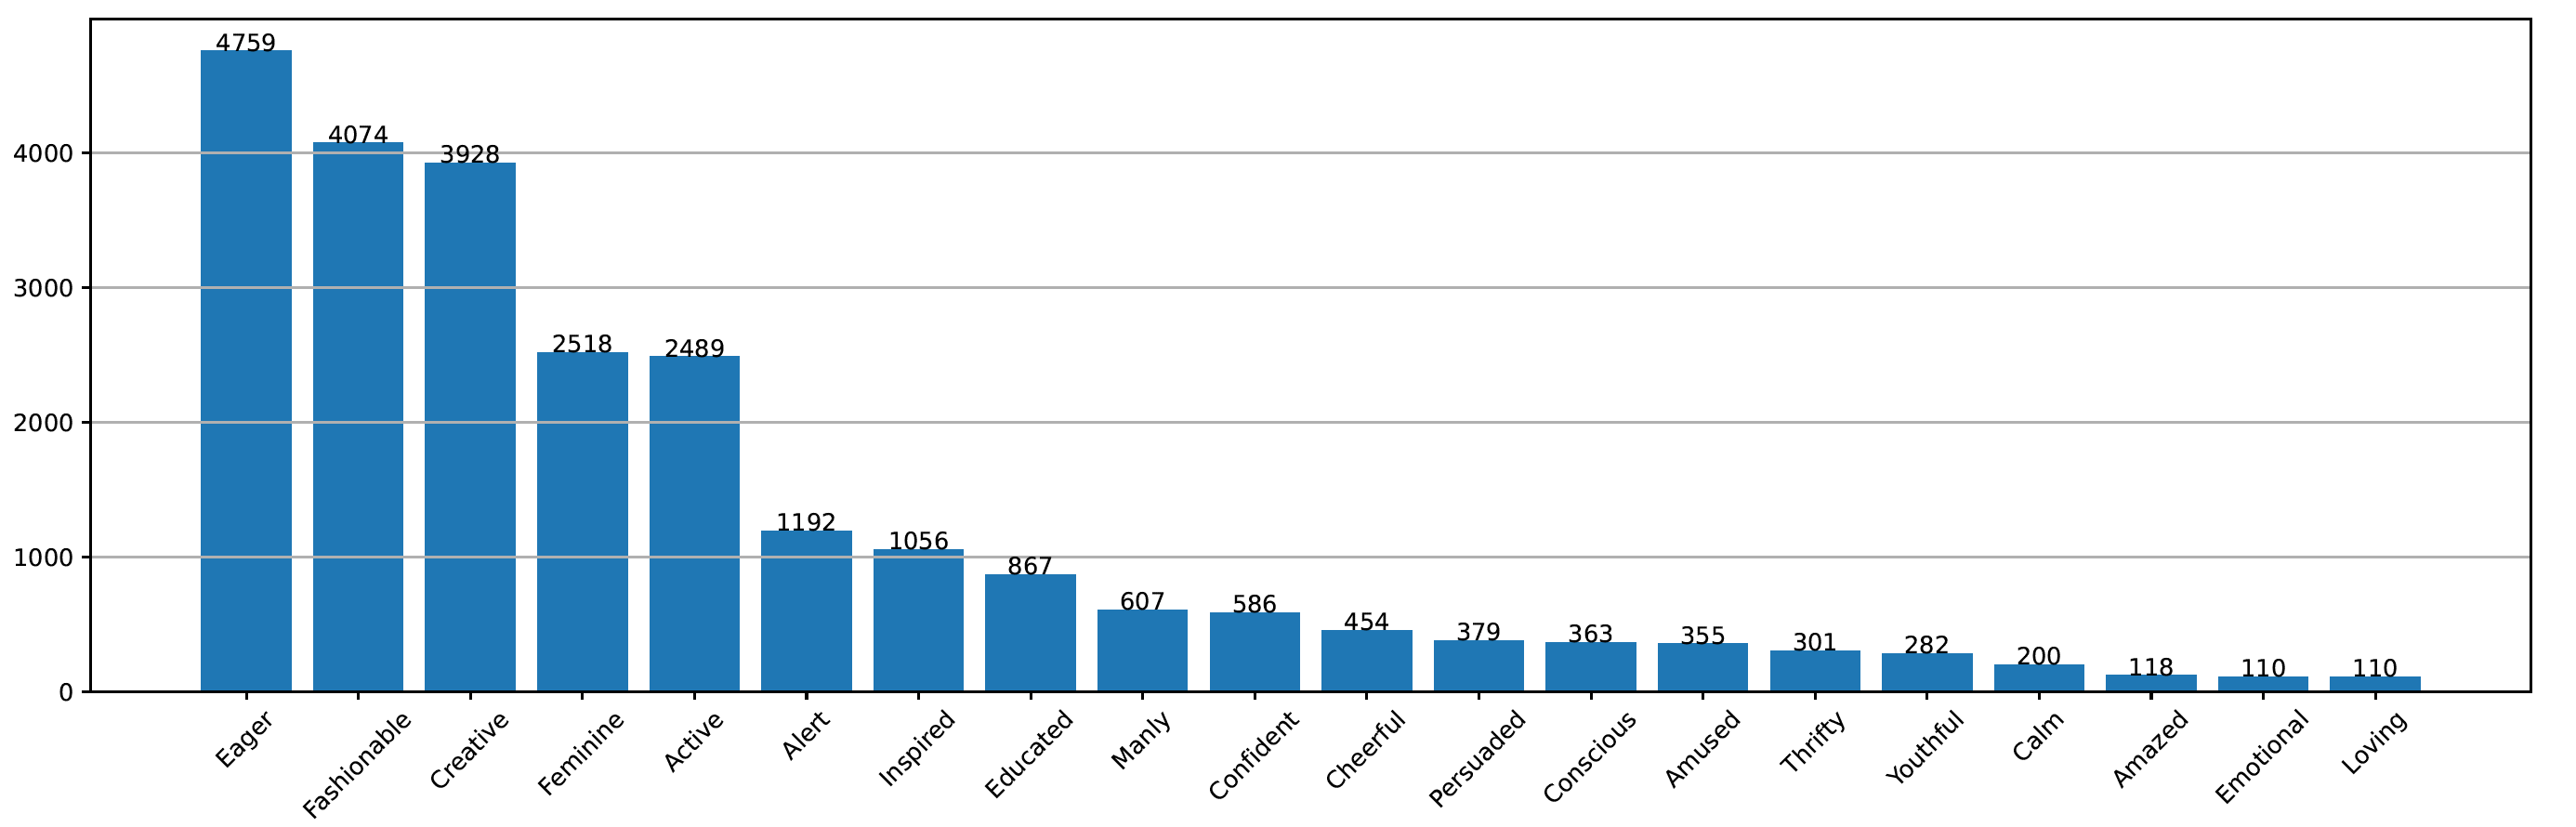
\includegraphics[width=8cm, height=10cm, keepaspectratio]{figures/dataset.eps}
\caption{Sentiment Label Distribution}
\label{fig:dataset}
\end{figure}

\section{Methodology} \label{sec:prop_method}

Before training, the images have to processed for denoising and their quality improved before loading it to model for classification. 

\subsection{Bilateral Filter}
For improving the quality of the images, a smoothing filter for images had to be employed. So, a bilateral filter was used to reduce noise while preserving edges in a non-linear manner. This filter works by calculating a weighted average of intensity values from surrounding pixels to replace the intensity of each pixel. The weight of each pixel is determined using a Gaussian distribution and it preserves sharp edges. The weights used in the filter are not solely based on the distance between pixels, but also take into consideration differences in radiometric properties such as color intensity and depth distance\cite{b15}.

\begin{figure}[htp]
\includegraphics[width=9cm, height=11cm, keepaspectratio]{figures/ads_bilateral.eps}
\caption{Bilateral Filter applied on Ads }
\label{fig:ads_bilateral}
\end{figure}

A bilateral filter is controlled by three parameters sigma(s), responsible for spatial region which smooths larger surfaces as we increase the spatial parameter, sigma(r) which tends to act like a Gaussian filter when it increases as the Gaussian range widens and d, which is the diameter of each pixel neighbourhood. It is quintessential to know that all other filters smudge the edges, while Bilateral Filtering retains them. When weights are multiplied together and if one of the weights is close to zero, no smoothing occurs. This can be demonstrated by using a large spatial Gaussian with a narrow range Gaussian, which results in limited smoothing despite the filter having a large spatial extent. The range weight ensures that the edges are preserved.

As shown in Fig.~\ref{fig:ads_bilateral}, after applying different values d, sigma(s) and sigma(r), it was determined that the pixel diameter of 9 along with sigma(s) and sigma(r) being 9 as well gave the best results. Following that, bilateral filters have been applied twice merely because of the fact that applying bilateral filters in iterations enhanced picture quality even more. Fig.~\ref{fig:ads_bilateral} depicts a significant change in the filtered image than the previous image i.e. the original image where the color banding or posterization, an ugly artifact that can be seen in digital images, has been notably reduced\cite{b16} and the final image is better than previous one. Another remarkable change was also witnessed which relates to compression artifacts, a distortion of media in images which is caused by lossy compression of media was also removed in the final image corroborating the efforts. 

\subsection{Pre-processing Techniques}
Pytorch provides various functional transformations that can be applied using the torchvision.transform module. They accept both PIL images and tensor images, although some transformations are PIL-only and some are tensor-only\cite{b17}. As these transformations require a parameter such as a factor by which an image can be transformed, therefore they cannot be applied to all images owing to the fact that all images are different.

\begin{figure}[htbp]
    \includegraphics[width=9cm, height=9cm, keepaspectratio]{figures/preprocessing_plots.eps}
    \caption{Pytorch Preprocessing Techniques}
    \label{fig:preprocessing_plots}
    \end{figure}

For example, a Hue transform that accepts an image along with a parameter, hue\_factor that ranges from [-0.5 to 0.5]. 0.5 and -0.5 give complete reversal of the hue channel in HSV space in positive and negative direction respectively whereas 0 means no shift. The same level of factor cannot be expected from other techniques such as sharpness or contrast etc. Hence, this parameter cannot be kept constant for all images as it will have a variable effect or appeal on different images. In the Fig.~\ref{fig:preprocessing_plots}, five random images have been selected and functional image processing techniques like hue transforms, gamma transforms, solarize transformations, sharpness, etc have been applied to reach a conclusion that all images bearing unique in their characteristics respond differently to functional transformations applied.

Even though brightness and contrast change show a potent outcome, a specific parameter cannot be kept for all images which points that this approach is to be handled in data augmentation where functions like AutoContrast and AutoBrightness have been applied. Histogram equalization, a popular technique for improving the contrast of images visibly failed to work for colored images. This technique was employed on a colored image which distorted colors and features such that it could not be considered as a viable pre-processing technique.

\begin{figure}[htbp] 
    \includegraphics[width=9cm, height=9cm, keepaspectratio]{figures/histogram_equalize.eps} 
    \caption{Histogram Equalization on Colored Image} 
    \label{fig:histogram_equalize}
    \end{figure}

Fig.~\ref{fig:histogram_equalize} shows the aftermath of histogram equalization on a colored image in detail where the image has been completely distorted in it's entirety and is difficult for any feature to be mapped.

\subsection{Data Augmentations Techniques}
Data augmentation plays a crucial role in completing the training requirements for deep learning models as deep learning models aren’t able to converge the network to an optimal solution because of the huge number of parameters needed to be tuned by the learning algorithm. It requires enormous amounts of data merely because of the fact that the deep learning algorithms start off with a poor initial state where weights are completely random and then optimization occurs using some gradient based optimization algorithm.  There are various ways to augment data using pytorch library such as RandomHorizontalFlip, RandomAdjustSharpness, etc that produce images with any random factor for creating image outputs that may be a possible scenario in the real world for exposing to variability and diversity in the image dataset. In Fig.~\ref{fig:RandomHorizontalFlip},~\ref{fig:RandomRotation30},~\ref{fig:ColorJitter},~\ref{fig:RandomAutocontrast} and~\ref{fig:RandomAdjustSharpness} data augmentation has been visualized using RandomHorizontalFlip, RandomRotation to 30 degrees, RandomColorJitter, RandomAutocontrast with factor as 5 and lastly RandomAdjustSharpness with sharpness factor as 2.

\begin{figure}[htbp] 
    \includegraphics[width=8cm, height=9cm, keepaspectratio]{figures/RandomHorizontalFlip.eps} 
    \caption{Data Augmentation using RandomHorizontalFlip} 
    \label{fig:RandomHorizontalFlip} 
    \end{figure}

\begin{figure}[htbp] 
    \includegraphics[width=8cm, height=9cm, keepaspectratio]{figures/RandomRotation30.eps} 
    \caption{Data Augmentation using RandomRotation} 
    \label{fig:RandomRotation30}
    \end{figure}

\begin{figure}[htbp] 
    \includegraphics[width=8cm, height=9cm, keepaspectratio]{figures/ColorJitter.eps} 
    \caption{Data Augmentation using ColorJitter} 
    \label{fig:ColorJitter} 
    \end{figure}

\begin{figure}[htbp] 
    \includegraphics[width=8cm, height=9cm, keepaspectratio]{figures/RandomAutocontrast.eps} 
    \caption{Data Augmentation using RandomAutocontrast} 
    \label{fig:RandomAutocontrast}
    \end{figure}

\begin{figure}[htbp] 
    \includegraphics[width=8cm, height=9cm, keepaspectratio]{figures/RandomAdjustSharpness.eps} 
    \caption{Data Augmentation using RandomAdjustSharpness} 
    \label{fig:RandomAdjustSharpness}
    \end{figure}
    


\subsection{Model Architectures} 
(\ref{tab:selArch}) Different backbone architectures were chosen to ensure that different types of Convolution blocks were tested for the advertisement data. Other selection criteria included the \textit{number of parameters} and \textit{GFLOPS}, important to keep track of the total training and evaluation time, and the \textit{top 5 classification accuracy} on the ImageNet 1K benchmark dataset. Finally, the following three
backbone architectures were chosen:

\begin{table}[htbp]
    \caption{Shortlisted Backbone Architectures.}
    \centering
    \begin{tabular}{p{1.5cm}|p{1cm}|p{1cm}|p{1.2cm}|p{1cm}}
    %\toprule
    \hline
    Arch. & Params (Mil.) & Layers & GFLOPS & Imagenet Acc.\\
    %\midrule
    \hline
    MobileNet V3 Large & 5.5 & 18 & 0.22 & 92.57\\
    %\midrule
    \hline
    EfficientNet B3 & 12.2 & 29 & 1.83 & 96.05\\
    %\midrule
    \hline
    Resnet 50 & 25.6 & 50 & 4.09 & 95.43\\
    %\bottomrule
    \hline
    \end{tabular}
    %\vspace{-1.5em}
    \label{tab:selArch}
  \end{table}

\textbf{ResNet 50}: A residual learning CNN with 50 layers that  are made possible by skip connections. Without these skip  connections, training such a deep network is not possible due to the vanishing gradient problem. The 50 layer variant was chosen to decrease training time while not compromising on the accuracy. This architecture had the highest trainable parameters, FLOPS and number of layers\cite{b18}.

\textbf{MobileNet V3 Large}: This model uses depthwise separable convolution  from MobileNet V2 along with squeezeexcitation blocks in residual layers  from MnasNet. This makes it really quick to train while still performing at par with other architectures. This architecture had the lowest trainable parameters and FLOPS among the three selected. Howard et al. Reference\cite{b19} also used network architecture search to find the most effective model. The large configuration was chosen to not compromise on the prediction accuracy.

\textbf{EfficientNet B3}: This model uses compound scaling to scale the model by 
depth, width and resolution. The B3 version was chosen to have faster training without compromising on the accuracy. Reference\cite{b20} This architecture performs the 
best among the selected on the Imagenet benchmark dataset while having half  the trainable parameters of Resnet50.


\subsection{Optimization Algorithm}
The Adam optimizer \cite{b21} is an adaptive learning rate optimization algorithm which was chosen as the optimizer for this study as it converges faster by integrating benefits of the RMSProp algorithm and momentum technique. It is also robust to hyperparameters but, requires tweaking of the learning rate depending on the task at hand. For this study, a learning rate of 0.01 and the original author recommend settings for $\beta_{1} = 0.9$, $\beta_{2} = 0.999$ and $\epsilon = 10^{-8}$ were used for the first and second order moment estimate as defined in \eqref{eq:adam1} and \eqref{eq:adam2} where $\beta_{1}$ and 
$\beta_{2}$ control the decay rates.

 \begin{equation}
 m_{t} = \beta_{1} \cdot m_{t-1} + (1 - \beta_{1}) \cdot g_{t}
 \label{eq:adam1}
 \end{equation}

 \begin{equation}
   v_{t} = \beta_{2} \cdot v_{t-1} + (1 - \beta_{2}) \cdot g_{t}^{2}
   \label{eq:adam2}
   \end{equation}

Further, the Cosine annealing \cite{b22} learning rate scheduler was used 
to reduce the learning rate as the training progressed down to an end point of 0.001. This 
would help us reduce the learning rate as training progressed, preventing us from overshooting the minima.

\section{Results} \label{sec:result}
\subsection{Experiment Setup}

First, training data with labels that were low in count were removed as described in \ref{sec:prop_method}. Then, the advertisement images were pre-processed using the bilateral filter described in \ref{sec:prop_method} before resizing them to the size - 384 * 384. The data was split into train, test and validation set in the 0.6:0.2:0.2 ratio and was stored in separate directories according to the defined PyTorch dataloader. 
Then, the mean and standard deviation of the dataset was calculated using the training dataset. All images were normalized before training using the dataloader with this calculated mean and standard deviation. The dataset used in this study presented the the multiclass, multilabel classification problem.  Thus, to make the model predict multiple labels, a sigmoid layer had to be added before the loss function to get 0 or 1 prediction for all the classes of the data. 
To achieve this, the BCEWITHLOGITSLOSS function of PyTorch was used as it combines the Sigmoid layer and the  binary cross entropy loss function in one single class. This makes 
theses operations more numerically stable than their separate counterparts \cite{23}.
The backbone architectures and their pre-trained weights were obtained directly from the 
torchvision library and the final classification layer was modified for our dataset of 20 classes. The pre-trained weights were chosen to be the IMAGENET1K\_V2 weights and only the last classification layer was fine-tuned. The rationale behind performing this type of 
shallow-tuning was that the Imagenet data is very similar to the advertisement images in our dataset. Additionally, the size of the selected dataset is small so deep-tuning might not work well. 

The batch size was fixed to 32 for all the models. While training, the best model by 
validation loss was saved to prevent the usage of overfit models for the test set analysis. The actual and predicted results from each epoch was also stored to calculate the F1 scores at each step of training. While calculating the F1 score, macro averaging 
was used to get an average score across classes. 

Initial training runs of the multilabel data produced a zero F1 score due to its highly imbalanced nature. To mitigate this, class wise weights were calculated and used with the loss function. This improved the F1 score quite considerably.

\begin{figure}[htbp]
    \centering
    \includegraphics[width=1\linewidth]{figures/metrics.eps}  
    \caption{Training \& Validation, F1 \& Loss plots for the three models.}
    %\vspace{-1em}
    \label{fig:acc_loss}
  \end{figure}


Finally, the best models from each of the three training runs validation loss were used 
to get the test set metrics that are displayed in \ref{table:test_metrics}. 
Per epoch training and validation F1 score and loss are provided in 
Fig.~\ref{fig:acc_loss}.

\subsection{Training Results}
From \ref{fig:acc_loss} it is clear that going from a smaller 
architecture to a bigger architecture, makes the model start to overfit earlier. 
The MobileNet model took the most number of epochs to reach the minima. The EfficientNet model performs the best for our dataset. However, all three models performed poorly. This shows that the compound scaling of EfficientNet gives good results for the advertisement dataset. The reason for poor performance overall could be due to a number of reasons. 
The had a high number of classes but the number of examples per class was very low.
Moreover, there was a high class imbalance problem. After looking at the images and 
the labels more closely, it was noticed that many images were poorly labeled and the 
labels contained quite a few synonyms. 

\begin{table}[htbp]
    \caption{F1 (higher is better), time per epoch in seconds (lower is better), and number of epochs to reach the best validation loss and F1 (lower is better) for the 3 models that were trained.}
    \centering
    \boldmath
    \begin{tabular}{p{2cm}|p{1cm}|p{1cm}|p{1.2cm}|p{1cm}}
    %\toprule
    \hline
    Model & \emph{F1} & \emph{Time} & \emph{F1 Epochs} & \emph{Loss Epochs}\\
    %\midrule
    \hline
    MobileNet V3 Large & 0.168 & \textbf{80s} & 50 & 98\\
    %\midrule
    \hline
    EfficientNet B3 & \textbf{0.189} & 153s & \textbf{5} & 90\\
    %\midrule
    \hline
    Resnet 50 & 0.179 & 89s & 10 & \textbf{0}\\
    %\bottomrule
    \hline
    \end{tabular}
    %\vspace{-1.5em}
    \label{tab:test_metrics}
    \end{table}

Looking at \ref{tab:test_metrics} it can be seen that the MobileNet architecture was 
the fastest to train per epoch. It took less time per epoch but, if number of epochs required to converge is considered, it does not train the fastest. The lowest validation set loss for ResNet was at epoch 0. This means that the model started overfitting right after the first epoch in terms of the loss. However, it took 10 epochs to converge on the F1 score.  EfficientNet model performed the best in terms of the overall F1 score on the test set. Another surprising observation is that the EfficientNet model takes the longest to train per epoch even though the number of trainable parameters is nowhere close to ResNet. 
Also, MobileNet isn't as fast to train as expected when compared to ResNet even though 
it has five times the learnable paramenters. This could be due to two reasons, 1. depthwise convolutions are not optimized in the version of PyTorch and CUDA used and 2. training is getting CPU bound due to the data augmentation before each training run which would take the same amount of time for all the models. 

\begin{figure}[htbp]
    \centering
    \includegraphics[width=1\linewidth]{figures/efficientnet_cm.eps}  
    \caption{Confusion Matrix for the EfficientNet model.}
    %\vspace{-1em}
    \label{fig:conf}
  \end{figure}

In Fig.~\ref{fig:conf} it can be seen that the model classifies the labels Fashionable, Feminine, and Eager the best which are the classes that have the most number of training examples. This shows that if we increase the training dataset size, the models could improve a lot.

\begin{figure}
    
    \subfloat[First Layer Activations]{\includegraphics[width = 1\linewidth]{figures/1_Layer_first.eps}}\\
    \subfloat[Middle Layer Activations]{\includegraphics[width = 1\linewidth]{figures/1_Layer_middle.eps}}\\
    \subfloat[Last layer Activations]{\includegraphics[width = 1\linewidth]{figures/1_Layer_last.eps}}
    \caption{GradCAM visualization for an Advertisement using the Efficientnet Model. Actual label - Eager}
    \label{fig:gradcam_1}
  \end{figure}

  \begin{figure}[htbp]
    \centering
    \includegraphics[width=1\linewidth]{figures/first_layer_filters.eps}  
    \caption{Filters of the first layer.}
    %\vspace{-1em}
    \label{fig:filters}
  \end{figure}

As the EfficientNet B3 model produced the best F1 score on the test set, it was used 
to generate the GradCAM visualizations to understand the model output. In Fig.~\ref{fig:gradcam_1} we can see that in the first layer of the network the model 
identifies prominent edges of the image. We can confirm this by looking at the filters of the first layer in Fig.~\ref{fig:filters}. Most of the filters look like they identify edges and corners. In the middle layer of the network, the model is looking at many different features but isn't looking at the most relavant features for that label. On the other hand, in the final layer of the network, the model looks only at the relavant features of the image depending on the current label. For example, here it is focusing on the player playing football for the 'Active' label. 

\begin{figure}
    
    \subfloat[First Layer Activations]{\includegraphics[width = 1\linewidth]{figures/2_Layer_first.eps}}\\
    \subfloat[Middle Layer Activations]{\includegraphics[width = 1\linewidth]{figures/2_Layer_middle.eps}}\\
    \subfloat[Last layer Activations]{\includegraphics[width = 1\linewidth]{figures/2_Layer_last.eps}}
    \caption{GradCAM visualization for an Advertisement using the Efficientnet Model. Actual label - Fashionable, Feminine, Persuaded}
    \label{fig:gradcam_2}
  \end{figure}

In Fig.~\ref{fig:gradcam_2}, the model focuses on the picture of the woman for the 'Feminine', 'Fashionable' and 'Cheerful' labels.

\begin{figure}
    
    \subfloat[First Layer Activations]{\includegraphics[width = 1\linewidth]{figures/9_Layer_first.eps}}\\
    \subfloat[Middle Layer Activations]{\includegraphics[width = 1\linewidth]{figures/9_Layer_middle.eps}}\\
    \subfloat[Last layer Activations]{\includegraphics[width = 1\linewidth]{figures/9_Layer_last.eps}}
    \caption{GradCAM visualization for an Advertisement using the Efficientnet Model. Actual label - Persuaded}
    \label{fig:gradcam_9}
  \end{figure}

In Fig.~\ref{fig:gradcam_9} We can see that the model correctly looked at the text 'Free' and classified the image as Thrifty however the actual label of persuaded was also in the top 4 predictions. This shows us that the model performs much better if we look at the images and generated outputs. The labels of the selected dataset are not completely correct making it difficult to evaluate the actual performance of the models. Visually looking at the gradcam visualizations and the predictions it is clear that the model is performing much better than what the F1 scores show.

\begin{figure}
    
    \subfloat[First Layer Activations]{\includegraphics[width = 1\linewidth]{figures/7_Layer_first.eps}}\\
    \subfloat[Middle Layer Activations]{\includegraphics[width = 1\linewidth]{figures/7_Layer_middle.eps}}\\
    \subfloat[Last layer Activations]{\includegraphics[width = 1\linewidth]{figures/7_Layer_last.eps}}
    \caption{GradCAM visualization for an Advertisement using the Efficientnet Model. Actual label - Creative}
    \label{fig:gradcam_7}
  \end{figure}


\section{Conclusion}

Understanding how humans perceive image advertisements could help improve the quality of these advertisements. Training a neural network model to predict the emaotions felt by humans towards different images is easy buy collecting the data is much more difficult. The low performance of the models in this study can be attributed to the low quality of the labels along with a lack of available training data. Even though the convolutional layers of the EfficientNet model were not fine-tuned, it was observed that the model could find relavant features in the image depending on the label. This shows that transfer learning is a powerful tool to train models and reduce turn around times. Transfer learning enables the use of deep learning models even when the amount of available data is very less. 

To improve the performance of the models, a number of things can be tried. Improving the labels of the available dataset can improve the models quite a bit. Additionally, getting more data would help the training effort by allowing the models to find patterns better. A long text description of how people feel when looking at different images could be an interesting take on this problem. Later, this text could be pre-processed using NLP models to create labels.

\begin{thebibliography}{00}
\bibitem{b1} https://www.oberlo.com/statistics/facebook-ad-revenue

\bibitem{b2} https://www.statista.com/statistics/266249/advertising-revenue-of-google/

\bibitem{b3} Mei, Tao, Xian-Sheng Hua, Linjun Yang, and Shipeng Li. "VideoSense: towards effective online video advertising." In Proceedings of the 15th ACM international conference on Multimedia, pp. 1075-1084. 2007.

\bibitem{b4} Girshick, Ross. "Fast r-cnn." In Proceedings of the IEEE international conference on computer vision, pp. 1440-1448. 2015.

\bibitem{b5} Szegedy, Christian, Wei Liu, Yangqing Jia, Pierre Sermanet, Scott Reed, Dragomir Anguelov, Dumitru Erhan, Vincent Vanhoucke, and Andrew Rabinovich. "Going deeper with convolutions." In Proceedings of the IEEE conference on computer vision and pattern recognition, pp. 1-9. 2015.

\bibitem{b6} Y. Donahue, Jeffrey, Lisa Anne Hendricks, Sergio Guadarrama, Marcus Rohrbach, Subhashini Venugopalan, Kate Saenko, and Trevor Darrell. "Long-term recurrent convolutional networks for visual recognition and description." In Proceedings of the IEEE conference on computer vision and pattern recognition, pp. 2625-2634. 2015.

\bibitem{b7} Vinyals, Oriol, Alexander Toshev, Samy Bengio, and Dumitru Erhan. "Show and tell: A neural image caption generator." In Proceedings of the IEEE conference on computer vision and pattern recognition, pp. 3156-3164. 2015.

\bibitem{b8} Borth, Damian, Rongrong Ji, Tao Chen, Thomas Breuel, and Shih-Fu Chang. "Large-scale visual sentiment ontology and detectors using adjective noun pairs." In Proceedings of the 21st ACM international conference on Multimedia, pp. 223-232. 2013.

\bibitem{b9} Chen, Tao, Felix X. Yu, Jiawei Chen, Yin Cui, Yan-Ying Chen, and Shih-Fu Chang. "Object-based visual sentiment concept analysis and application." In Proceedings of the 22nd ACM international conference on Multimedia, pp. 367-376. 2014.

\bibitem{b10} Chen, Tao, Damian Borth, Trevor Darrell, and Shih-Fu Chang. "Deepsentibank: Visual sentiment concept classification with deep convolutional neural networks." arXiv preprint arXiv:1410.8586 (2014).

\bibitem{b11} Hussain, Zaeem, Mingda Zhang, Xiaozhong Zhang, Keren Ye, Christopher Thomas, Zuha Agha, Nathan Ong, and Adriana Kovashka. "Automatic understanding of image and video advertisements." In Proceedings of the IEEE conference on computer vision and pattern recognition, pp. 1705-1715. 2017.

\bibitem{b12} Vedula, Nikhita, Wei Sun, Hyunhwan Lee, Harsh Gupta, Mitsunori Ogihara, Joseph Johnson, Gang Ren, and Srinivasan Parthasarathy. "Multimodal content analysis for effective advertisements on youtube." In 2017 IEEE international conference on data mining (ICDM), pp. 1123-1128. IEEE, 2017.

\bibitem{b13} Madhok, Rishi, Shashank Mujumdar, Nitin Gupta, and Sameep Mehta. "Semantic understanding for contextual in-video advertising." In Proceedings of the AAAI Conference on Artificial Intelligence, vol. 32, no. 1. 2018.

\bibitem{b14} Zhang, Huaizheng, Yong Luo, Qiming Ai, Yonggang Wen, and Han Hu. "Look, read and feel: Benchmarking ads understanding with multimodal multitask learning." In Proceedings of the 28th ACM International Conference on Multimedia, pp. 430-438. 2020.

\bibitem{b15} https://en.wikipedia.org/wiki/Bilateral\_filter

\bibitem{b16} https://www.willgibbons.com/color-banding/

\bibitem{b17} https://pytorch.org/vision/stable/transforms.html

\bibitem{b18} He, Kaiming, Xiangyu Zhang, Shaoqing Ren, and Jian Sun. "Deep residual learning for image recognition." In Proceedings of the IEEE conference on computer vision and pattern recognition, pp. 770-778. 2016.

\bibitem{b19} Howard, Andrew, Mark Sandler, Grace Chu, Liang-Chieh Chen, Bo Chen, Mingxing Tan, Weijun Wang et al. "Searching for mobilenetv3." In Proceedings of the IEEE/CVF international conference on computer vision, pp. 1314-1324. 2019.

\bibitem{b20} Tan, Mingxing, and Quoc Le. "Efficientnet: Rethinking model scaling for convolutional neural networks." In International conference on machine learning, pp. 6105-6114. PMLR, 2019.

\bibitem{21} Kingma, Diederik P., and Jimmy Ba. "Adam: A method for stochastic optimization." arXiv preprint arXiv:1412.6980 (2014).

\bibitem{22} Loshchilov, Ilya, and Frank Hutter. "Sgdr: Stochastic gradient descent with warm restarts." arXiv preprint arXiv:1608.03983 (2016).

\bibitem{23} https://pytorch.org/docs/stable/generated/torch.nn.BCEWithLogitsLoss.html

\end{thebibliography}

\end{document}
